\chapter{Implementation}
\label{cha:impl}

Chapter 4

\section{Pre-Processing}

Figure \ref{bbdatatable} shows the raw format of the Britain Breathing dataset. There are a few procedures that need doing before it can be used in a hotspot identification algorithm. Before I had a web page running with the capability of displaying geographical data I relied on Tableau to visualise and alter all datasets.\\ 

The Britain Breathing dataset in it's raw format contained entries from all over the world. I could have decided to leave them on as I could centre the map on the UK so only those who where curious enough to pan around the rest of the globe would see these extra points. But that's more of a novel thing. At the time of pre-processing, I thought the extra points might affect some of the hotspot algorithm calculations such as global averages so I decided to remove all points that are not on mainland UK or in Northern and the Republic of Ireland.\\

\begin{SCfigure}
\label{fig:RTv1}
\caption{Figure \ref{fig:RTv1} : Britain Breathing dataset before processing}\\
\centering
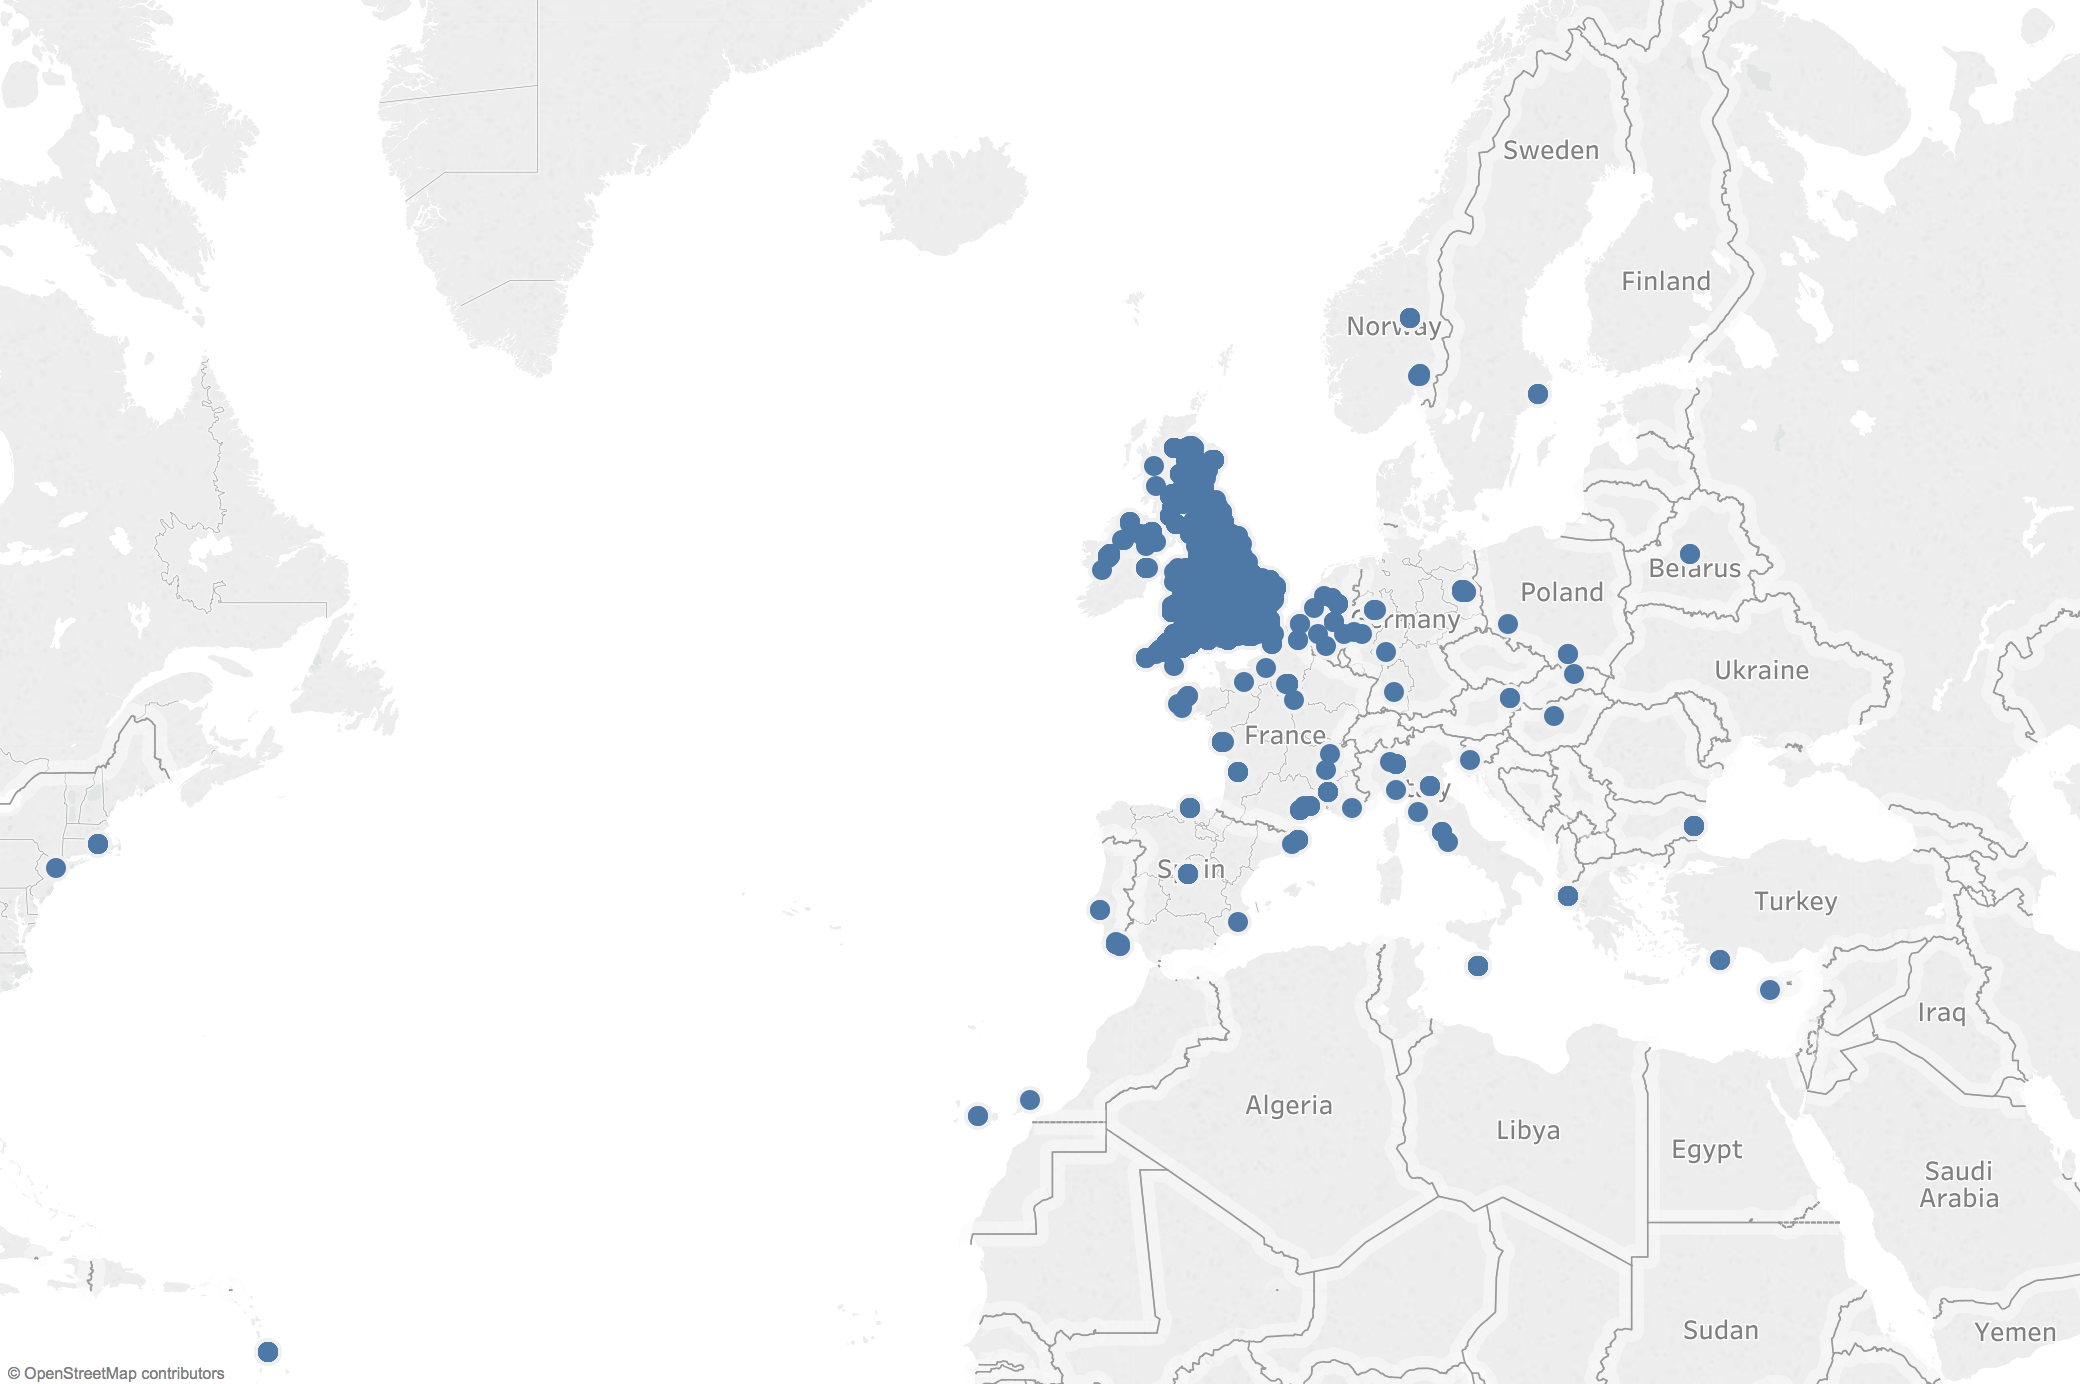
\includegraphics[width=0.75\textwidth]{tableuaeverywhere}
\centering
\end{SCfigure}\\

Approximately 2.7\% of entries had a null value for one of the attributes. 96\% of these nulls were  whether or not the user had existing hay fever or asthma, I decided to remove each of these records entirely, I could also have decided set the attribute to 0 or 1 but I wanted to avoid fabricating data to keep any conclusions made using the data valid.\\

Whilst using Tableau to visualise the data in the early stages of development I noticed there were a few clusters of points in virtually the same place. For example, there is a user in the north of Scotland who used the app at times multiple times a day to record her allergy symptoms. This resulted a fairly large set of results for a very sparsely populated area. I decided to remove most of the results for this person as the area was identified as a hotspot. I think there could be arguments for keeping the data but I don't think that allowing one persons enthusiasm to track her allergy problems makes sense for a project aimed at producing results that could be used to aid research.\\

Once the data has been improved from its raw format, it is stored on the server as a .JSON file. I decided against using a database to store my datasets as I wanted to avoid having to convert to and from JSON. The end application ended up being rather CPU intensive so this decision turned out very well.

\subsection{Road Traffic}

The Road Traffic dataset in its raw format was far from being usable.\\

As you can see from figure \ref{fig:rt} the first version of the Road Traffic dataset was way too dense. I needed the dataset to be able to be displayed with the heatmap generated from the Britain Breathing dataset to be visible behind the Road Traffic data in order to compare the two. There were too many roads of very short spans cluttering the view of the heatmap.\\

\begin{SCfigure}
\label{fig:rt}
\caption{Figure \ref{fig:rt} : First attempt at displaying the Road Traffic data}\\
\centering
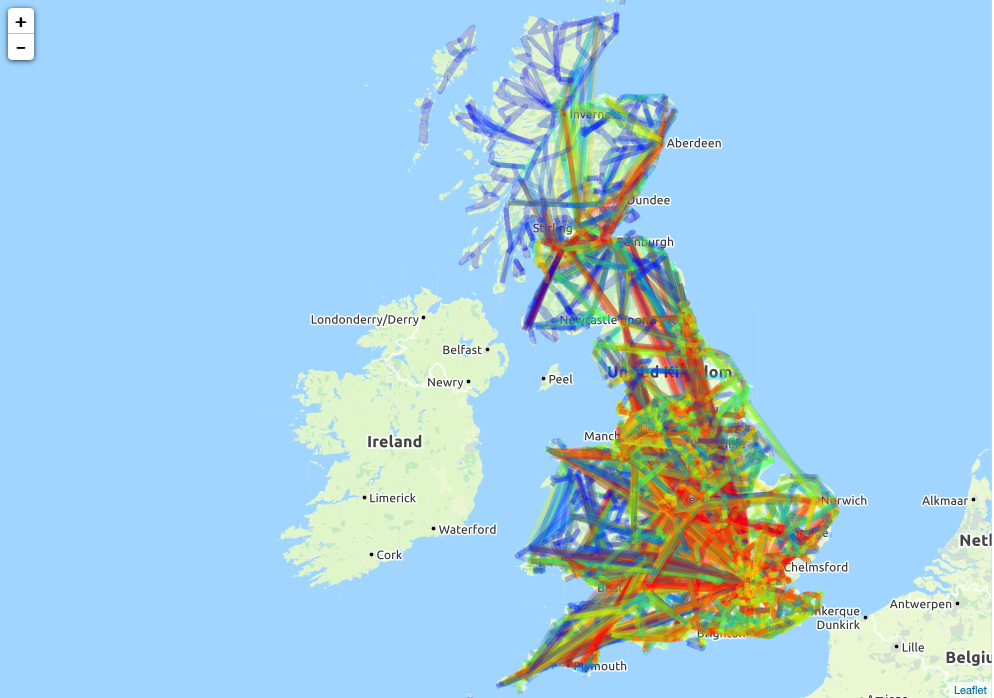
\includegraphics[width=0.75\textwidth]{RoadTrafficv1}
\centering
\end{SCfigure}\\

Upon zooming in and inspecting the data I also found that some roads were stored incorrectly in the dataset. Around 10 roads were stored as having their junction before and junction after being the ends of the road. Roads like the A1 can be as long as 396 miles so errors can cause big problems \cite{longestRoad}. In the case of the A1, the entire road was displayed as a deep red indicating a high volume of traffic. For the majority of the A1, this would be true but there are areas of the road that are not particularly busy so they're being wrongly represented. \\

I created a java program to process the data before being stored on the server. Java was chosen purely because I have most experience with it and I knew exactly how to read and write files, making it a good choice for pre-processing the Road Traffic data. For each entry, counts are discarded if the length of the distance between the junction before and the junction after is longer than 200km or if the road is shorter than 5km and has a density in the lower 5\% of the data. Removing the smaller roads like this removes the mess of small roads with negligible traffic in places like the north of Scotland. These roads don't provide much information and therefore do not help to find hotspots, they just make the map look cluttered.\\

\section{Heatmap Generation}

Once the data is in a useable format and condition, I need to display that data on a map. In this section will explain the steps taken to get to point where I have a allergy symptom hotspot represented as a heatmap using Leaflet.\\

The Britain Breathing JSON file is loaded from the server. An instance of a HotspotArray is instantiated with parameters including x and y values for the dimension of the desired map resolution. The resolution values are used to create a two dimensional array with sizes [x][y]. This array is used to divide the area of the UK into distinct square areas. See figure \ref{fig:hh} for a small scale example.

\begin{SCfigure}
\label{fig:hh}
\caption{Figure \ref{fig:hh} : A [5][7] resolution example}\\
\centering
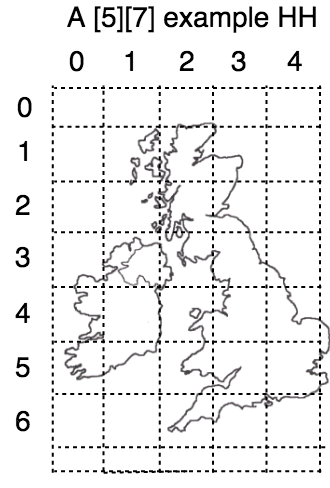
\includegraphics[width=0.4\textwidth]{hh5x7}
\centering
\end{SCfigure}\\

By default, I used a 500 by 500 resolution as I found this gives enough of a resolution so that you can't see the square boundaries at any zoom level but also keeps the map easy to use in calculations. The alternative here would have been to use something like the UK Council boundaries, but I didn't like how they looked on the map. This was mainly due to the fact that dividing the map by Councils meant that you don't get precise enough information on specific allergy symptoms hotspots. A hotspot in a City such as Inverness would cause a massive area including tiny three or four house villages in the middle of the Scottish highlands to be indicated as being a "hotspot".\\

For each entry in the processed dataset;

\begin{enumerate}
    \item Add entry to the Hotspot Array. The latitude and longitude of the entry is used to map to an index in the array. For example, a location in the top left of the map would map to [0][0], bottom right would map to [499][499] etc. 
    \item If there is already a value in the Hotspot Array, add to the total count and update the average for the square area. Otherwise, add to the total count and calculate average.
\end{enumerate}

The next step after filling the Hotspot Array with the data is to do some hotspot identification.

\subsection{Spatial Autocorrelation}

Determining if an area is a hotspot or not can be done using Spatial Autocorrelation (SA). SA is a way of giving a numerical value to the degree of which an area is similar to nearby areas \cite{autocor} . A high positive value indicates that an area has a statistically significant value when compared to its neighbours and should be indicated as a hotspot. A low positive or negative value indicates that it is likely that the value is randomly clustered. A high negative value shows a cluster of low values. See Figure \ref{fig:autcor2}\\

\begin{SCfigure}
\label{fig:autocor2}
\caption{Figure \ref{fig:autocor2} : Spatial Autocorrelation}\\
\centering
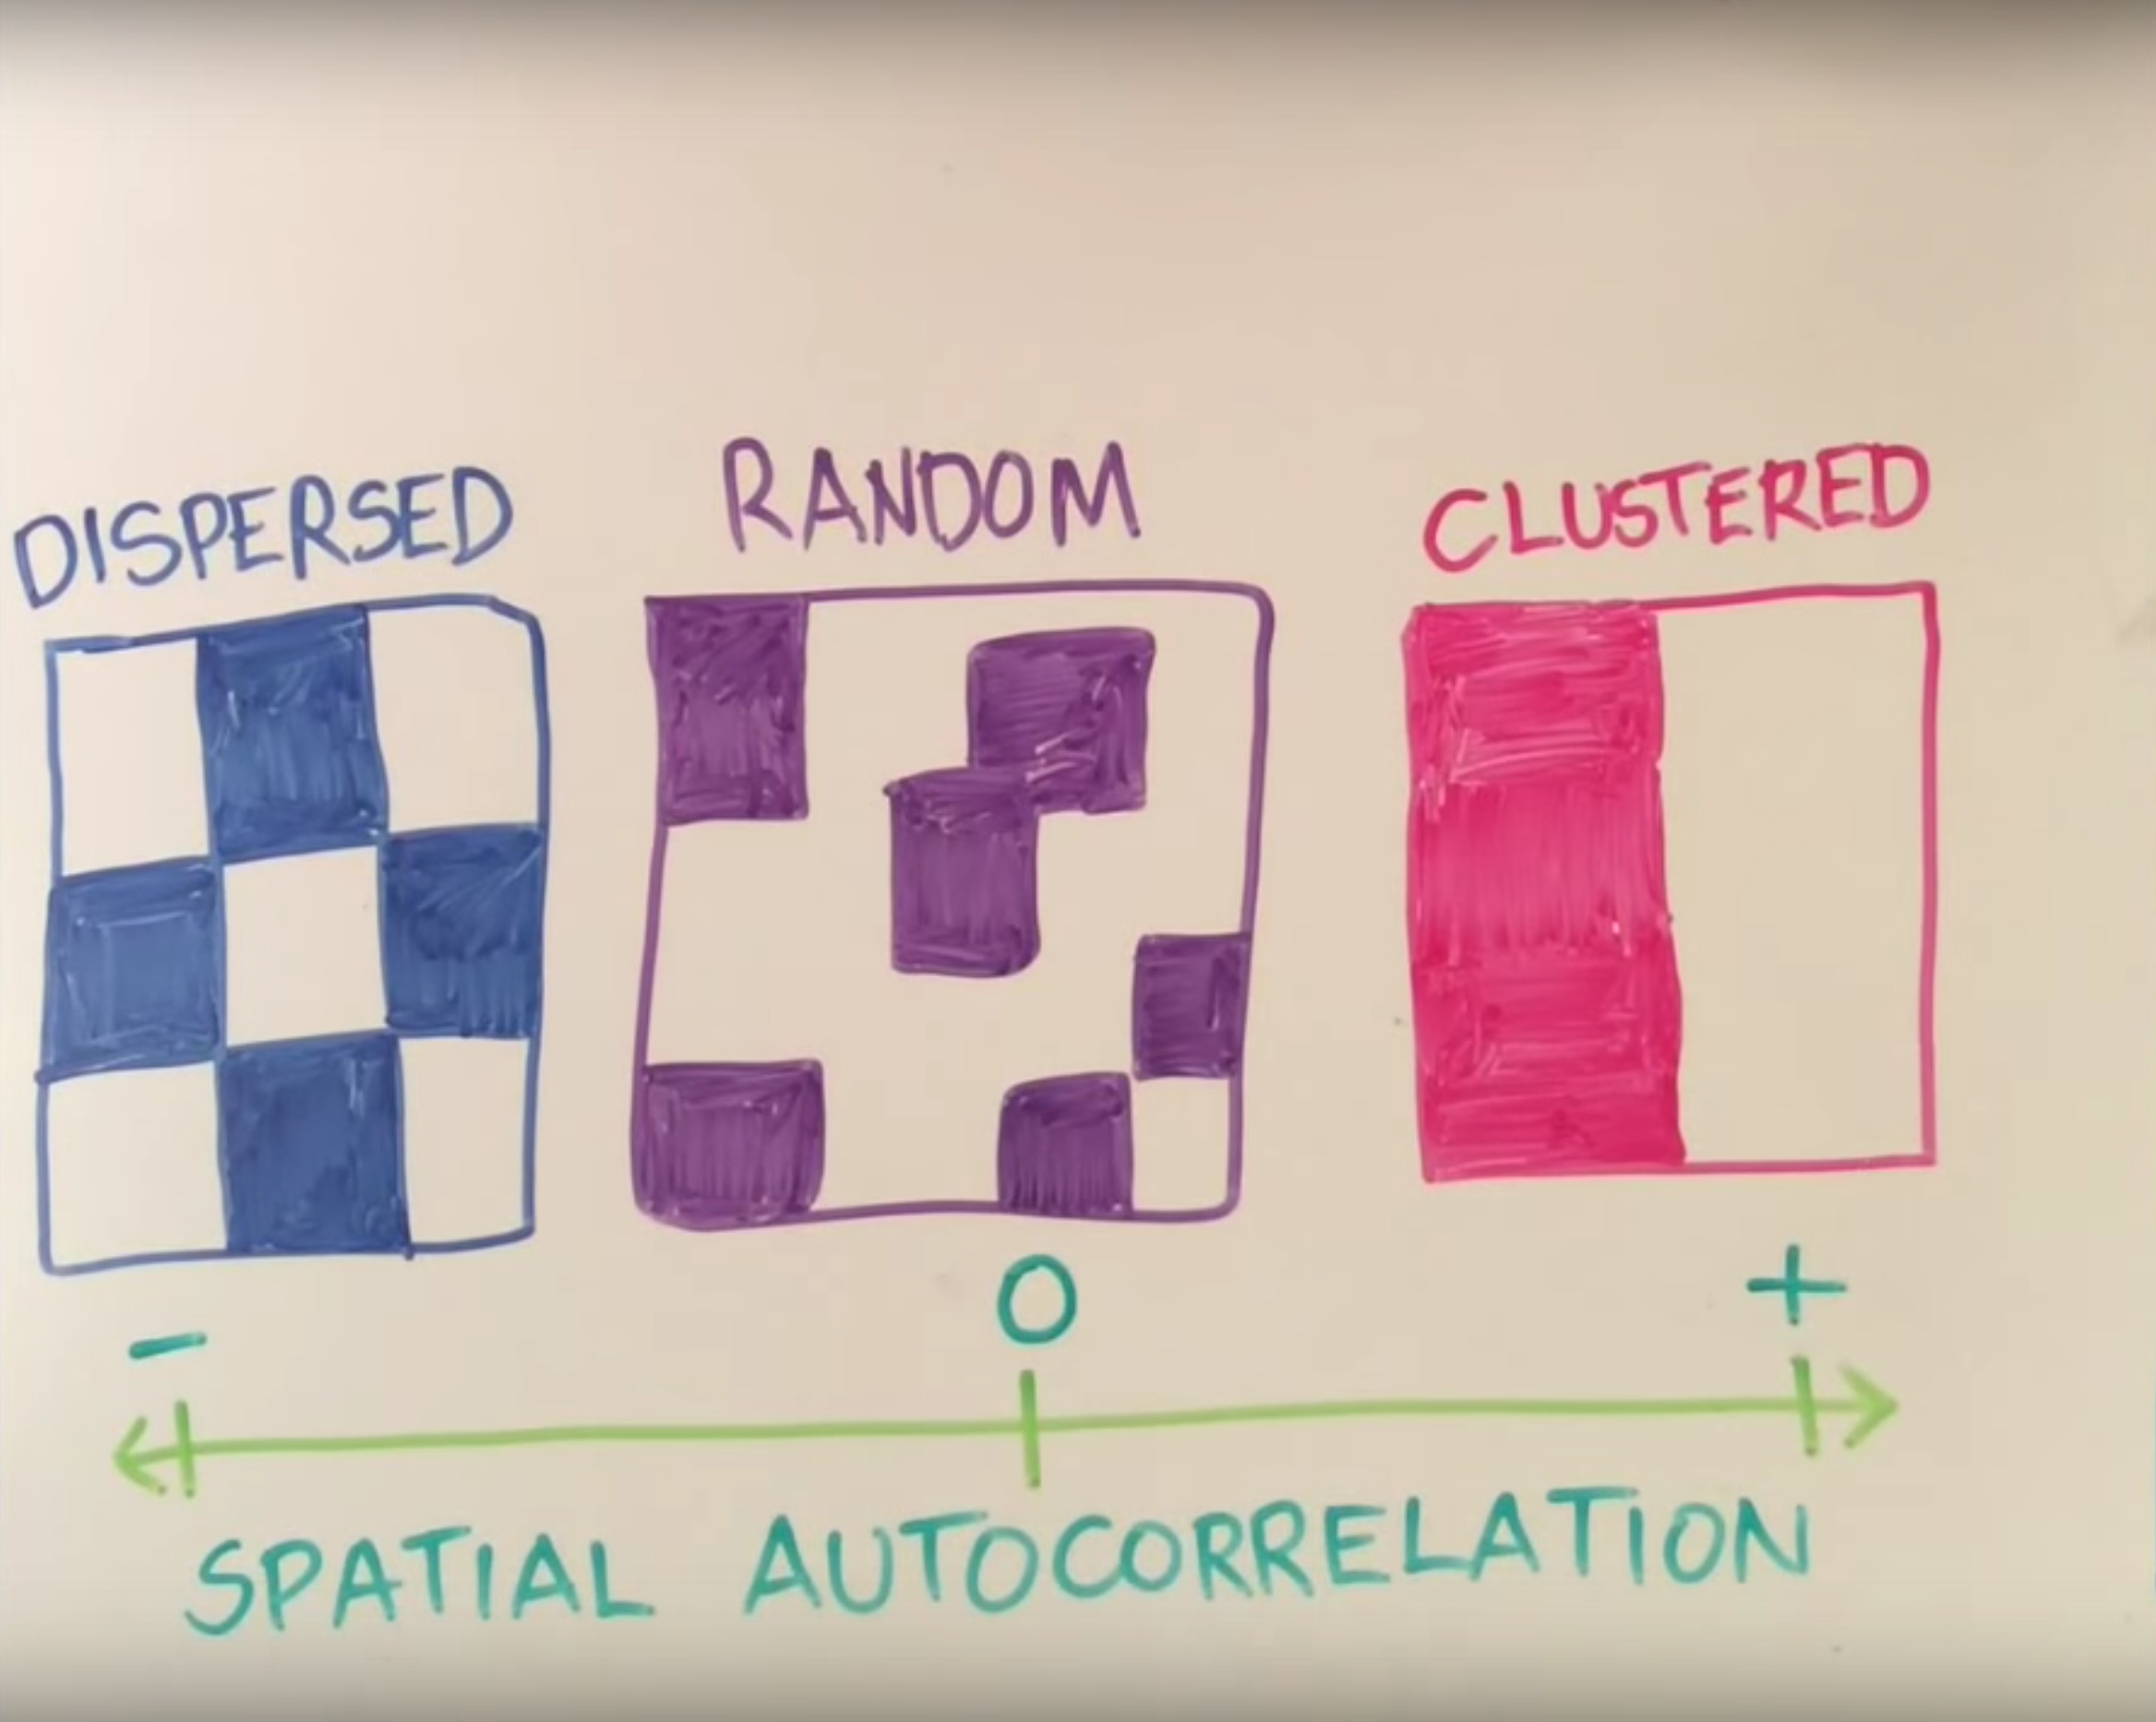
\includegraphics[width=0.4\textwidth]{autocor2}
\centering
\end{SCfigure}\\

If an area has a high positive value then we can consider that area a hotspot. So if an area has lots of high positive values they should accumulate to generate a higher allergy symptom score. Equally, if an area has a few high positive values, a few small absolute values and a few large negative values, the algorithm should take this into account and not label the area as a hotspot.\\

A good but effective way of doing this is just to average the z-scores for the area and then use this score in the heatmap.

\subsection{Distance Calculations}

Calculating the statistical significance of values, and whether or not they are related to nearby values involves calculating the distance between points.\\

There are many ways of calculating the distance between two dimensional points and it's not a particularly interesting topic so I'll keep it brief. I decided to use the Manhattan distance as shown below \ref{dia:manhat}.\\

dist (x, y)  = $\sqrt{ \sum_{i=1}^{n}(x_i - y_i)^2$ }\label{dia:manhat}\\

\subsection{Using distances}

The closer two points are, the more they will affect each other. It would not be correct to say that a cluster of allergy symptoms in Manchester should have any affect at all on those in Liverpool. So I need a way of using these distances to calculate how much to take the surrounding areas into account. Or as Waldo Tobler's first law of Geography puts it. "everything is related to everything else, but near things are more related than distant things." \ref{waldo}\\






\subsection{Getis-Ord}

\subsection{Speed issues and the Solution}

\section{Allergy Score}

\section{Smart Data Tool}

Now that I have some good datasets and I understand how they effect each other, I need a way o

How relate dataset to specific allergies and symptoms